%% Submissions for peer-review must enable line-numbering
%% using the lineno option in the \documentclass command.
%%
%% Preprints and camera-ready submissions do not need
%% line numbers, and should have this option removed.
%%
%% Please note that the line numbering option requires
%% version 1.1 or newer of the wlpeerj.cls file, and
%% the corresponding author info requires v1.2

\documentclass[fleqn,10pt]{wlpeerj} % for preprint submissions

% ZNK -- Adding headers for pandoc

\setlength{\emergencystretch}{3em}
\providecommand{\tightlist}{
\setlength{\itemsep}{0pt}\setlength{\parskip}{0pt}}
\usepackage{lipsum}
\usepackage[unicode=true]{hyperref}
\usepackage{longtable}

\usepackage{color}
\usepackage{fancyvrb}
\newcommand{\VerbBar}{|}
\newcommand{\VERB}{\Verb[commandchars=\\\{\}]}
\DefineVerbatimEnvironment{Highlighting}{Verbatim}{commandchars=\\\{\}}
% Add ',fontsize=\small' for more characters per line
\usepackage{framed}
\definecolor{shadecolor}{RGB}{248,248,248}
\newenvironment{Shaded}{\begin{snugshade}}{\end{snugshade}}
\newcommand{\AlertTok}[1]{\textcolor[rgb]{0.94,0.16,0.16}{#1}}
\newcommand{\AnnotationTok}[1]{\textcolor[rgb]{0.56,0.35,0.01}{\textbf{\textit{#1}}}}
\newcommand{\AttributeTok}[1]{\textcolor[rgb]{0.77,0.63,0.00}{#1}}
\newcommand{\BaseNTok}[1]{\textcolor[rgb]{0.00,0.00,0.81}{#1}}
\newcommand{\BuiltInTok}[1]{#1}
\newcommand{\CharTok}[1]{\textcolor[rgb]{0.31,0.60,0.02}{#1}}
\newcommand{\CommentTok}[1]{\textcolor[rgb]{0.56,0.35,0.01}{\textit{#1}}}
\newcommand{\CommentVarTok}[1]{\textcolor[rgb]{0.56,0.35,0.01}{\textbf{\textit{#1}}}}
\newcommand{\ConstantTok}[1]{\textcolor[rgb]{0.00,0.00,0.00}{#1}}
\newcommand{\ControlFlowTok}[1]{\textcolor[rgb]{0.13,0.29,0.53}{\textbf{#1}}}
\newcommand{\DataTypeTok}[1]{\textcolor[rgb]{0.13,0.29,0.53}{#1}}
\newcommand{\DecValTok}[1]{\textcolor[rgb]{0.00,0.00,0.81}{#1}}
\newcommand{\DocumentationTok}[1]{\textcolor[rgb]{0.56,0.35,0.01}{\textbf{\textit{#1}}}}
\newcommand{\ErrorTok}[1]{\textcolor[rgb]{0.64,0.00,0.00}{\textbf{#1}}}
\newcommand{\ExtensionTok}[1]{#1}
\newcommand{\FloatTok}[1]{\textcolor[rgb]{0.00,0.00,0.81}{#1}}
\newcommand{\FunctionTok}[1]{\textcolor[rgb]{0.00,0.00,0.00}{#1}}
\newcommand{\ImportTok}[1]{#1}
\newcommand{\InformationTok}[1]{\textcolor[rgb]{0.56,0.35,0.01}{\textbf{\textit{#1}}}}
\newcommand{\KeywordTok}[1]{\textcolor[rgb]{0.13,0.29,0.53}{\textbf{#1}}}
\newcommand{\NormalTok}[1]{#1}
\newcommand{\OperatorTok}[1]{\textcolor[rgb]{0.81,0.36,0.00}{\textbf{#1}}}
\newcommand{\OtherTok}[1]{\textcolor[rgb]{0.56,0.35,0.01}{#1}}
\newcommand{\PreprocessorTok}[1]{\textcolor[rgb]{0.56,0.35,0.01}{\textit{#1}}}
\newcommand{\RegionMarkerTok}[1]{#1}
\newcommand{\SpecialCharTok}[1]{\textcolor[rgb]{0.00,0.00,0.00}{#1}}
\newcommand{\SpecialStringTok}[1]{\textcolor[rgb]{0.31,0.60,0.02}{#1}}
\newcommand{\StringTok}[1]{\textcolor[rgb]{0.31,0.60,0.02}{#1}}
\newcommand{\VariableTok}[1]{\textcolor[rgb]{0.00,0.00,0.00}{#1}}
\newcommand{\VerbatimStringTok}[1]{\textcolor[rgb]{0.31,0.60,0.02}{#1}}
\newcommand{\WarningTok}[1]{\textcolor[rgb]{0.56,0.35,0.01}{\textbf{\textit{#1}}}}


\usepackage{lipsum}
\usepackage{booktabs}
\usepackage{longtable}
\usepackage{array}
\usepackage{multirow}
\usepackage{wrapfig}
\usepackage{float}
\usepackage{colortbl}
\usepackage{pdflscape}
\usepackage{tabu}
\usepackage{threeparttable}
\usepackage{threeparttablex}
\usepackage[normalem]{ulem}
\usepackage{makecell}
\usepackage{xcolor}

\title{Visualisation of Brain Statistics with R-package \texttt{ggseg}}

\author[1]{Athanasia M. Mowinckel}

\corrauthor[1]{Athanasia M. Mowinckel}{\href{mailto:a.m.mowinckel@psykologi.uio.no}{\nolinkurl{a.m.mowinckel@psykologi.uio.no}}}
\author[1]{Didac Vidal Piñeiro}


\affil[1]{Center for Lifespan Changes in Brain and Cognition, Univeristy of Oslo, PO. box 1094 Blindern, 0317 Oslo, Norway}


%
% \author[1]{First Author}
% \author[2]{Second Author}
% \affil[1]{Address of first author}
% \affil[2]{Address of second author}
% \corrauthor[1]{First Author}{f.author@email.com}

% 
\usepackage{natbib}
\bibliographystyle{plainnat}

\begin{abstract}
The abstract of the article. It can also be on \emph{multiple} lines.
% Dummy abstract text. Dummy abstract text. Dummy abstract text. Dummy abstract text. Dummy abstract text. Dummy abstract text. Dummy abstract text. Dummy abstract text. Dummy abstract text. Dummy abstract text. Dummy abstract text.
\end{abstract}

\begin{document}

\flushbottom
\maketitle
\thispagestyle{empty}

\hypertarget{introduction}{%
\section{Introduction}\label{introduction}}

Neuroscientific analysis usually requires the use of multiple tools to analyse, visualise, and summarise data.
This often makes the process of preparing results for publication laborious, as results must be exported and imported in various formats.
In neuroimaging, images of probands' brains are collected and merged together to provide three dimensional representations.
Much of the neuroimaging analyses are not necessarily done on the individual voxel level (3-dimensional pixels), but rather on pre-defined brain segmentations, called brain atlases.
These brain atlases are plentiful and represent different ways of segmenting the brain into functionally or structurally similar regions (\citet{dkt}).
The use of these is wide-spread, as these atlases provide larger meaningful divisions of the brain.
While neuroimaging analyses on the voxel-level are usually computed by special software for such analyses, analyses of brain atlas data is usually done in standard statistical software, like R (\citet{R}), python (\citet{python}), or MATLAB (\citet{MATLAB}).

A key part of understanding and disseminating analysis results, is the visualization of these in a meaningful way.
With regards to results from brain atlas analyses, it is most meaningfully represented if projected onto a representation of the brain, rather than other common types of charts (like bar-charts) accompanied by a diagram of the brain label positions.
Each atlas has its own labelling depending on what is meaningful for the type of segmentation it is based on.
As such, for the reader to fully understand a bar chart with atlas labels, they need to be very familiar with the location of each label to have a clear comprehension of the results.
A projection directly onto a brain shape, eases the readability of the results for the reader, and provides clear point of reference even if the used atlas is unfamiliar.

There are several tools that aid R-users in plotting neuroimaging data directly through R using the grammar of graphics as implemented in ggplot2 (\citet{ggplot}), such as ggBrain (\citet{ggBrain}) and ggneuro (\citet{ggneuro}; see neuroconductor \citeyearpar{neuroconductor} for curated neuroimaging packages for R).
These are based on plotting imaging files, not results from analyses of brain atlases.
Here we introduce the ggseg-package for visualizing results from brain atlas analyses.
The ggseg-package was developed to create templates that others might use to project their brain atlas results on to.
While its plotting functions are what the users are drawn to, it is the pre-compiled number of data sets for different brain atlases that provides the real functionality needed for this visualization.
The package also includes functions to plot atlases in tri-surface mesh plots using plotly (\citet{plotly}).

\hypertarget{brain-atlas-selection}{%
\subsection{Brain atlas selection}\label{brain-atlas-selection}}

There is a multitude of brain atlases to chose from, all with different purposes and segmented based on different criteria.
We have initially focused on commonly used and well-established atlases with manageable numbers of segmentations.
The ggseg-package thus features data for two well-established parcellations, as implemented in the neuroimaging software Freesurfer \citep{fischl:99}; dkt and aseg.
The Desikan-Killany cortical atlas (dkt; \citet{dkt}) and the Automatic Segmentation of Subcortical Structures (aseg; \citet{aseg}) together cover all grey matter of the brain, and are commonly used in analyses elucidating the associations between thickness, volume, or area of these segments and mental health and cognitive function.

While functions and base data can be found in the main \texttt{ggseg}-package, a companion package called \texttt{ggsegExtra} has numerous other atlases, and is continuously expanded.
We encourage the community to help build and expand the atlases available, and to create a repository of established and often used atlases.
A summary of all available atlases may be found in Table \ref{tab:atlasTab}, where in addition to the two default atlases, ggsegExtra has another 12 atlases.
The \href{https://github.com/LCBC-UiO/ggseg/wiki}{ggseg wiki} currently has two different ways you may create and supply atlases to the package as 2D polygons.
Work is being done to include instructions on 3D-mesh plot contributions also.
The package includes functions like \texttt{as\_ggseg\_atlas()} and \texttt{as\_ggseg3d\_atlas()} to aid users in testing and making custom atlases.

\begin{table}[t]

\caption{\label{tab:atlasTab}Table of currently available atlases in either ggseg or ggsegExtra R-package. Most atlases have both polygon and mesh atlases, but the mesh atlases are somewhat easier to create and are thus more plentiful. }
\centering
\begin{tabular}{lllll}
\toprule
Package & Title & Item & Mesh & Polygon\\
\midrule
 & Desikan-Killiany Cortical Atlas & dkt & No & Yes\\
\cmidrule{2-5}
 & \makecell[l]{Desikan-Killiany Cortical Atlas - tri-\\surf mesh Mesh data for the Desikan-\\Killany Cortical atlas, with 40 regions\\in on the cortical surface of the brain.} & dkt & Yes & No\\
\cmidrule{2-5}
\multirow{-3}{*}{\raggedright\arraybackslash ggseg} & \makecell[l]{Freesurfer automatic subcortical\\segmentation of a brain volume} & aseg & Yes & Yes\\
\cmidrule{1-5}
 & Desterieux cortical parcellations & desterieux & Yes & No\\
\cmidrule{2-5}
 & Harvard-Oxford Cortical atlas & hoCort & No & Yes\\
\cmidrule{2-5}
 & Parcellation from a midsagittal slice & midsagittal & No & Yes\\
\cmidrule{2-5}
 & Parcellation from JHU & jhu & No & Yes\\
\cmidrule{2-5}
 & Parcellation from of JHU & jhu & Yes & No\\
\cmidrule{2-5}
 & Parcellation from of white matter & icbm & Yes & No\\
\cmidrule{2-5}
 & Parcellation from of white matter & tracula & Yes & Yes\\
\cmidrule{2-5}
 & \makecell[l]{Parcellation from the Human Connectome\\Project} & glasser & Yes & Yes\\
\cmidrule{2-5}
 & \makecell[l]{Schaefer 17 Resting-state Cortical\\Parcellations} & schaefer17 & Yes & No\\
\cmidrule{2-5}
 & \makecell[l]{Schaefer 7 Resting-state Cortical\\Parcellations} & schaefer7 & Yes & No\\
\cmidrule{2-5}
 & \makecell[l]{Yeo 17 Resting-state Cortical\\Parcellations} & yeo17 & Yes & Yes\\
\cmidrule{2-5}
\multirow{-12}{*}{\raggedright\arraybackslash ggsegExtra} & \makecell[l]{Yeo 7 Resting-state Cortical\\Parcellations} & yeo7 & Yes & Yes\\
\bottomrule
\end{tabular}
\end{table}

\hypertarget{tutorial}{%
\section{Tutorial}\label{tutorial}}

The aim of this tutorial is to familiarize the reader with the main package functions and the general use of the package.\\
It will cover the two main functions: \texttt{ggseg()} which plots 2D polygons, and \texttt{ggseg3d()} which plots tri-surface mesh plots.

\hypertarget{plotting-polygon-data}{%
\subsection{Plotting polygon data}\label{plotting-polygon-data}}

The function to plot two-dimensional polygon data is the \texttt{ggseg}-function.
This function will automatically plot the dkt-atlas by default (see Figure \ref{fig:init}).
As this function is a wrapper for \texttt{geom\_polygon} from \texttt{ggplot2} it can be built upon like all ggplot objects.
The plot is kept as simple as possible, with as little extra information to ggplot as possible.
This is done for it to be easy to extend the plot with the many ggplot options available.

\begin{Shaded}
\begin{Highlighting}[]
\KeywordTok{library}\NormalTok{(ggseg)}
\KeywordTok{library}\NormalTok{(tidyverse)}
\KeywordTok{ggseg}\NormalTok{()}
\end{Highlighting}
\end{Shaded}

\begin{figure}
\centering

\includegraphics{draft_1_files/figure-latex/init-1.pdf}
\caption{\label{fig:init}By default \texttt{ggseg} will plot the dkt atlas in shaded polygons.}
\end{figure}

Because of the way \texttt{ggseg} is implemented, you should be able to safely use the function together with other ggplot functions, like themes, scales, and such (see Figure \ref{fig:void}).
There are many extra options to ggseg, to alter the plot as you wish.

\begin{Shaded}
\begin{Highlighting}[]
\NormalTok{p1 <-}\StringTok{ }\KeywordTok{ggseg}\NormalTok{(}\DataTypeTok{position =} \StringTok{"stacked"}\NormalTok{) }\OperatorTok{+}\StringTok{ }
\StringTok{  }\KeywordTok{theme_dark}\NormalTok{() }\OperatorTok{+}\StringTok{ }
\StringTok{  }\KeywordTok{labs}\NormalTok{(}\DataTypeTok{title=}\StringTok{"dkt"}\NormalTok{, }\DataTypeTok{subtitle =} \StringTok{"dark theme"}\NormalTok{)}
\NormalTok{p2 <-}\StringTok{ }\KeywordTok{ggseg}\NormalTok{(}\DataTypeTok{position =} \StringTok{"stacked"}\NormalTok{) }\OperatorTok{+}\StringTok{ }
\StringTok{  }\KeywordTok{theme_classic}\NormalTok{() }\OperatorTok{+}\StringTok{ }
\StringTok{  }\KeywordTok{labs}\NormalTok{(}\DataTypeTok{title=}\StringTok{"dkt"}\NormalTok{, }\DataTypeTok{subtitle =} \StringTok{"classic theme"}\NormalTok{)}

\CommentTok{# Combine plots}
\NormalTok{pp <-}\StringTok{ }\NormalTok{cowplot}\OperatorTok{::}\KeywordTok{plot_grid}\NormalTok{(p1, p2, }\DataTypeTok{nrow =} \DecValTok{2}\NormalTok{)}

\NormalTok{p3 <-}\StringTok{ }\KeywordTok{ggseg}\NormalTok{(}\DataTypeTok{atlas=}\NormalTok{aseg) }\OperatorTok{+}\StringTok{ }
\StringTok{  }\KeywordTok{labs}\NormalTok{(}\DataTypeTok{title=}\StringTok{"aseg"}\NormalTok{, }\DataTypeTok{subtitle =} \StringTok{"default theme"}\NormalTok{)}

\CommentTok{# Create a subplot grid}
\NormalTok{cowplot}\OperatorTok{::}\KeywordTok{plot_grid}\NormalTok{(pp, p3, }\DataTypeTok{nrow =} \DecValTok{1}\NormalTok{)}
\end{Highlighting}
\end{Shaded}

\begin{figure}
\centering
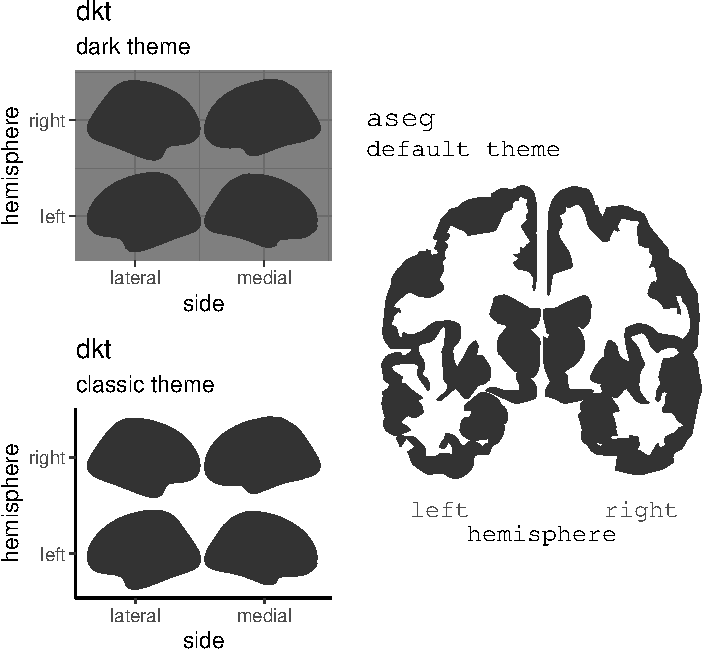
\includegraphics{draft_1_files/figure-latex/void-1.pdf}
\caption{\label{fig:void}ggseg plots can be used with most standard scales, themes and such that work with ggplot. The special ggseg options for hemispheres, view etc. depend on the atlas used, and some options are only available for certain atlases. There is no `lateral' or `medial' views of subcortical atlases.}
\end{figure}

You can stack the hemispheres, view only the medial or lateral side, choose either or both of the hemispheres, or a combination of any of these (see Figure \ref{fig:stacked}).
The possibilities of altering the plot depends on the atlas used.
There are generally more options available for cortical atlases than subcortical ones, as the atlases have more meaningful ways of viewing the polygons.
Subcortical atlases also tend to have structures that span the hemispheres or other typically used referece points of the brain, and as such it is more difficult to label all segments as either, e.g., left or right.

\begin{Shaded}
\begin{Highlighting}[]
\NormalTok{lat <-}\StringTok{ }\KeywordTok{ggseg}\NormalTok{(}\DataTypeTok{view =} \StringTok{"medial"}\NormalTok{) }\OperatorTok{+}\StringTok{ }
\StringTok{  }\KeywordTok{labs}\NormalTok{(}\DataTypeTok{title =} \StringTok{"Medial view"}\NormalTok{)}
\NormalTok{left <-}\StringTok{ }\KeywordTok{ggseg}\NormalTok{(}\DataTypeTok{hemisphere =} \StringTok{"left"}\NormalTok{) }\OperatorTok{+}\StringTok{ }
\StringTok{  }\KeywordTok{labs}\NormalTok{(}\DataTypeTok{title =} \StringTok{"Left hemi."}\NormalTok{)}
\NormalTok{pp <-}\StringTok{ }\NormalTok{cowplot}\OperatorTok{::}\KeywordTok{plot_grid}\NormalTok{(lat, left, }\DataTypeTok{nrow=}\DecValTok{2}\NormalTok{)}

\NormalTok{combo <-}\StringTok{ }\KeywordTok{ggseg}\NormalTok{(}\DataTypeTok{view =} \StringTok{"medial"}\NormalTok{,}
      \DataTypeTok{hemisphere =} \StringTok{"left"}\NormalTok{) }\OperatorTok{+}\StringTok{ }
\StringTok{  }\KeywordTok{labs}\NormalTok{(}\DataTypeTok{title =} \StringTok{"Combination"}\NormalTok{)}

\NormalTok{cowplot}\OperatorTok{::}\KeywordTok{plot_grid}\NormalTok{(pp, combo, }\DataTypeTok{nrow=}\DecValTok{1}\NormalTok{)}
\end{Highlighting}
\end{Shaded}

\begin{figure}
\centering
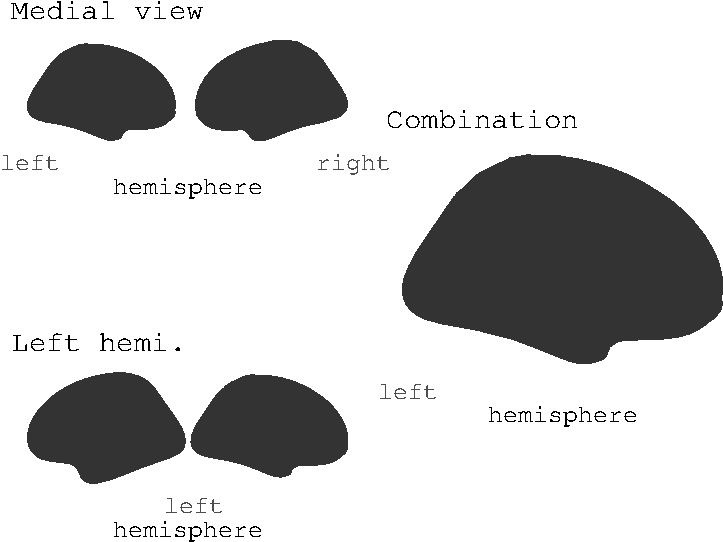
\includegraphics{draft_1_files/figure-latex/stacked-1.pdf}
\caption{\label{fig:stacked}There are several ggseg-special options that may be supplied to control how the plots looks and is organised. Top left: plot using medial view. Bottom left: plot using left hemisphere. Right: plot combining both the options.}
\end{figure}

\hypertarget{using-own-data-with-fill-and-colour}{%
\subsubsection{Using own data with fill and colour}\label{using-own-data-with-fill-and-colour}}

\texttt{ggseg} accepts any argument you can supply to \texttt{geom\_polygon} and therefore is easy to work with for those familiar with ggplot functionality.
Standard arguments like \texttt{fill} to flood the segments with a colour, or \texttt{colour} to colour the edges around the segments are typical arguments to provide to the function either as a single value or within the ggplot mapping option \texttt{aes}.

\begin{Shaded}
\begin{Highlighting}[]
\KeywordTok{ggseg}\NormalTok{(}\DataTypeTok{mapping=}\KeywordTok{aes}\NormalTok{(}\DataTypeTok{fill =}\NormalTok{ area), }\DataTypeTok{colour=}\StringTok{"black"}\NormalTok{) }\OperatorTok{+}\StringTok{ }
\StringTok{  }\KeywordTok{scale_fill_brain}\NormalTok{(}\StringTok{"dkt"}\NormalTok{) }\OperatorTok{+}
\StringTok{  }\KeywordTok{theme}\NormalTok{(}\DataTypeTok{legend.justification=}\KeywordTok{c}\NormalTok{(}\DecValTok{1}\NormalTok{,}\DecValTok{0}\NormalTok{),}
        \DataTypeTok{legend.position=}\StringTok{"bottom"}\NormalTok{,}
        \DataTypeTok{legend.text =} \KeywordTok{element_text}\NormalTok{(}\DataTypeTok{size =} \DecValTok{5}\NormalTok{)) }\OperatorTok{+}
\StringTok{  }\KeywordTok{guides}\NormalTok{(}\DataTypeTok{fill =} \KeywordTok{guide_legend}\NormalTok{(}\DataTypeTok{ncol =} \DecValTok{3}\NormalTok{))}
\end{Highlighting}
\end{Shaded}

\begin{figure}
\centering
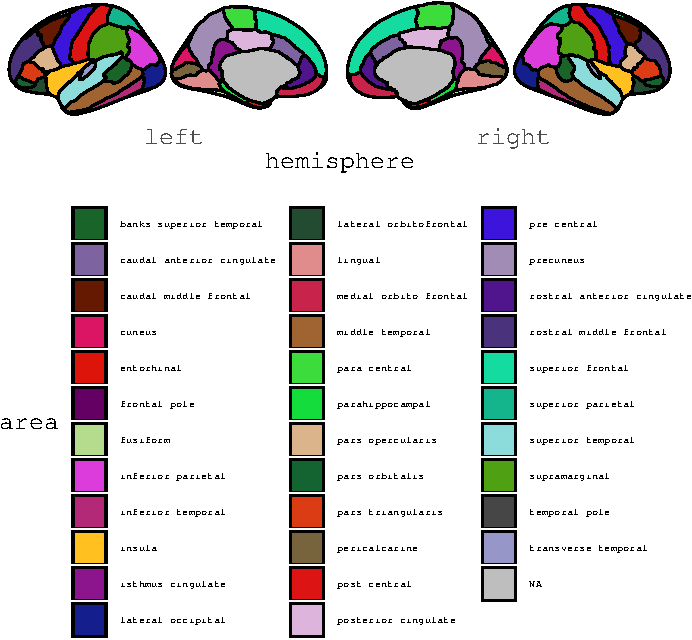
\includegraphics{draft_1_files/figure-latex/fill-1.pdf}
\caption{\label{fig:fill}Supplying `area' to the fill option in ggseg, will use the column `area' from the accompanying dataset to create a discrete colour palette over the segments in the atlas.}
\end{figure}

Typically you would want each area to have a different colour, corresponding to some descriptive or inference statistic that has been computed.
The bulk of the package originates not in its functions, but in the datasets that accompany the package.
There is one dataset per atlas, which contains key information regarding the atlas, and coordinates for the segment polygons of the atlas.
Before setting up the data from the statistics to project onto the segments, looking at the atlas datasets might help understand what the data needs to look like, or avoid looking like.

\small

\begin{Shaded}
\begin{Highlighting}[]
\NormalTok{dkt}
\end{Highlighting}
\end{Shaded}

\begin{verbatim}
## # A tibble: 80 x 6
##    atlas area               hemi  side    label             ggseg          
##    <chr> <chr>              <chr> <chr>   <chr>             <list>         
##  1 dkt   superior temporal  left  lateral lh_superiortempo~ <tibble [1,494~
##  2 dkt   pre central        left  lateral lh_precentral     <tibble [1,314~
##  3 dkt   post central       left  lateral lh_postcentral    <tibble [1,164~
##  4 dkt   rostral middle fr~ left  lateral lh_rostralmiddle~ <tibble [1,194~
##  5 dkt   insula             left  lateral lh_insula         <tibble [870 x~
##  6 dkt   superior parietal  left  lateral lh_superiorparie~ <tibble [480 x~
##  7 dkt   inferior temporal  left  lateral lh_inferiortempo~ <tibble [906 x~
##  8 dkt   lateral occipital  left  lateral lh_lateraloccipi~ <tibble [738 x~
##  9 dkt   lateral orbitofro~ left  lateral lh_lateralorbito~ <tibble [528 x~
## 10 dkt   superior frontal   left  lateral lh_superiorfront~ <tibble [420 x~
## # ... with 70 more rows
\end{verbatim}

\normalsize

The column `label' was added to the atlas for easy matching with the output from Freesurfer statistics tables.
The data is in long-format, meaning each segment has its own row, meaning the data you wish to project onto the segments also need to be in long-format.
As data directly from Freesurfer comes in wide-format, this requires some extra wranling.

\begin{Shaded}
\begin{Highlighting}[]
\NormalTok{freesurfer_stats <-}\StringTok{ }\KeywordTok{data.frame}\NormalTok{(}
  \DataTypeTok{id =} \KeywordTok{c}\NormalTok{(}\DecValTok{10}\OperatorTok{:}\DecValTok{12}\NormalTok{),}
  \DataTypeTok{lh_superiortemporal =} \KeywordTok{c}\NormalTok{(}\FloatTok{3.32}\NormalTok{, }\FloatTok{4.1}\NormalTok{, }\FloatTok{3.5}\NormalTok{),}
  \DataTypeTok{lh_precentral =} \KeywordTok{c}\NormalTok{(}\FloatTok{2.3}\NormalTok{, }\FloatTok{2.5}\NormalTok{, }\FloatTok{2.1}\NormalTok{),}
  \DataTypeTok{lh_rostralmiddlefrontal =} \KeywordTok{c}\NormalTok{(}\FloatTok{3.3}\NormalTok{, }\FloatTok{3.2}\NormalTok{, }\FloatTok{3.1}\NormalTok{)}
\NormalTok{  )}
\NormalTok{freesurfer_stats}
\end{Highlighting}
\end{Shaded}

\begin{verbatim}
##   id lh_superiortemporal lh_precentral lh_rostralmiddlefrontal
## 1 10                3.32           2.3                     3.3
## 2 11                4.10           2.5                     3.2
## 3 12                3.50           2.1                     3.1
\end{verbatim}

\begin{Shaded}
\begin{Highlighting}[]
\NormalTok{freesurfer_long <-}\StringTok{ }\NormalTok{freesurfer_stats }\OperatorTok\StringTok{ }
\StringTok{  }\KeywordTok{gather}\NormalTok{(label, thickness, }\OperatorTok{-}\NormalTok{id)}
\NormalTok{freesurfer_long}
\end{Highlighting}
\end{Shaded}

\begin{verbatim}
##   id                   label thickness
## 1 10     lh_superiortemporal      3.32
## 2 11     lh_superiortemporal      4.10
## 3 12     lh_superiortemporal      3.50
## 4 10           lh_precentral      2.30
## 5 11           lh_precentral      2.50
## 6 12           lh_precentral      2.10
## 7 10 lh_rostralmiddlefrontal      3.30
## 8 11 lh_rostralmiddlefrontal      3.20
## 9 12 lh_rostralmiddlefrontal      3.10
\end{verbatim}

This data can now be used directly with the \texttt{ggseg} function, as the \texttt{label} column corresponds in name and content with the \texttt{label} column in the atlas data of dkt.
The data \textbf{must} include a column that has the same name at atleast \emph{some} data matching the values in the corresponding column in the atlas data.
In the next example we create some data with 4 rows, and an `area' and `p' column.
The \texttt{ggseg} function will recognise the matching column `area', and merge the supplied data into the atlas using \texttt{dplyr} joins.
We use the \texttt{p} column as the column flooding the segment with colour.

\begin{Shaded}
\begin{Highlighting}[]
\NormalTok{someData =}\StringTok{ }\KeywordTok{data.frame}\NormalTok{(}
  \DataTypeTok{area =} \KeywordTok{c}\NormalTok{(}\StringTok{"transverse temporal"}\NormalTok{, }\StringTok{"insula"}\NormalTok{,}
           \StringTok{"pre central"}\NormalTok{,}\StringTok{"superior parietal"}\NormalTok{), }
  \DataTypeTok{p =} \KeywordTok{sample}\NormalTok{(}\KeywordTok{seq}\NormalTok{(}\DecValTok{0}\NormalTok{,.}\DecValTok{5}\NormalTok{,.}\DecValTok{001}\NormalTok{), }\DecValTok{4}\NormalTok{),}
  \DataTypeTok{stringsAsFactors =} \OtherTok{FALSE}\NormalTok{)}

\NormalTok{p <-}\StringTok{ }\KeywordTok{ggseg}\NormalTok{(}\DataTypeTok{.data=}\NormalTok{someData, }\DataTypeTok{mapping=}\KeywordTok{aes}\NormalTok{(}\DataTypeTok{fill=}\NormalTok{p))}
\NormalTok{p}
\end{Highlighting}
\end{Shaded}

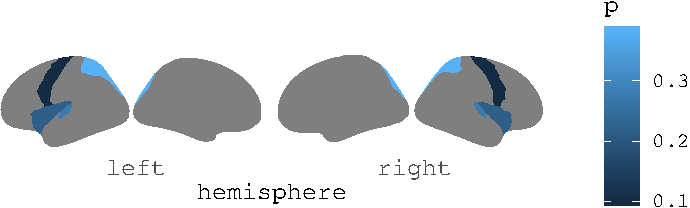
\includegraphics{draft_1_files/figure-latex/datasupp-1.pdf}

We can also change how this looks, by various ggplot functions, like scales, labs, themes and such.

\begin{Shaded}
\begin{Highlighting}[]
\NormalTok{p }\OperatorTok{+}
\StringTok{  }\KeywordTok{theme_void}\NormalTok{() }\OperatorTok{+}
\StringTok{  }\KeywordTok{scale_fill_gradient}\NormalTok{(}\DataTypeTok{low=}\StringTok{"firebrick"}\NormalTok{,}\DataTypeTok{high=}\StringTok{"goldenrod"}\NormalTok{) }\OperatorTok{+}
\StringTok{  }\KeywordTok{labs}\NormalTok{(}\DataTypeTok{title=}\StringTok{"A nice plot title"}\NormalTok{, }\DataTypeTok{fill=}\StringTok{"p-value"}\NormalTok{)}
\end{Highlighting}
\end{Shaded}

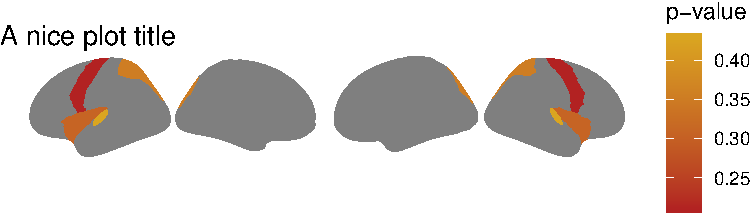
\includegraphics{draft_1_files/figure-latex/datasupp2-1.pdf}

If the results are only in one hemisphere, but you still want to plot both of them, make sure your data.fame includes the column \texttt{hemi} with either ``right'' or ``left'' for this to happen.

\begin{Shaded}
\begin{Highlighting}[]
\NormalTok{someData}\OperatorTok{$}\NormalTok{hemi =}\StringTok{ "right"}

\KeywordTok{ggseg}\NormalTok{(}\DataTypeTok{.data=}\NormalTok{someData, }\DataTypeTok{colour=}\StringTok{"white"}\NormalTok{,}\DataTypeTok{mapping=}\KeywordTok{aes}\NormalTok{(}\DataTypeTok{fill=}\NormalTok{p)) }\OperatorTok{+}
\StringTok{  }\KeywordTok{theme_void}\NormalTok{() }\OperatorTok{+}
\StringTok{  }\KeywordTok{scale_fill_gradient}\NormalTok{(}\DataTypeTok{low=}\StringTok{"firebrick"}\NormalTok{,}\DataTypeTok{high=}\StringTok{"goldenrod"}\NormalTok{) }\OperatorTok{+}
\StringTok{  }\KeywordTok{labs}\NormalTok{(}\DataTypeTok{title=}\StringTok{"Another nice plot title"}\NormalTok{)}
\end{Highlighting}
\end{Shaded}

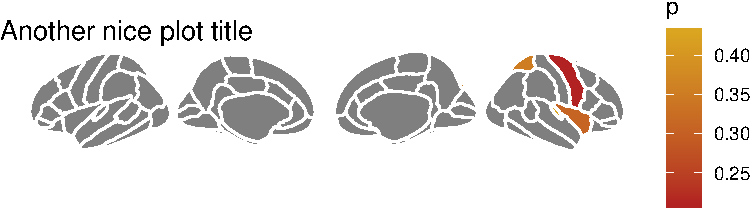
\includegraphics{draft_1_files/figure-latex/datasuppX-1.pdf}

\hypertarget{creating-subplots}{%
\subsubsection{Creating subplots}\label{creating-subplots}}

If your data has different statistics for different groups, and you want to plot them all, we can use ggplot's \texttt{facet\_wrap} or \texttt{facet\_grid} for that.
The data needs to be in long format for this to work, as needed by ggplot, meaning the data from the groups should appear in seperate rows in the data, not in separate columns. Secondly, the data needs to be grouped using \texttt{dplyr}'s \texttt{group\_by} function \emph{before} providing the data to the \texttt{ggseg} function.
The ggseg-function will detect if the data is grouped, and perform the necessary steps for the \texttt{facet}'s to work when they are applied later.

\begin{Shaded}
\begin{Highlighting}[]
\NormalTok{someData =}\StringTok{ }\KeywordTok{data.frame}\NormalTok{(}
  \DataTypeTok{area =} \KeywordTok{rep}\NormalTok{(}\KeywordTok{c}\NormalTok{(}\StringTok{"transverse temporal"}\NormalTok{, }\StringTok{"insula"}\NormalTok{,}
               \StringTok{"pre central"}\NormalTok{,}\StringTok{"superior parietal"}\NormalTok{),}\DecValTok{2}\NormalTok{), }
  \DataTypeTok{p =} \KeywordTok{sample}\NormalTok{(}\KeywordTok{seq}\NormalTok{(}\DecValTok{0}\NormalTok{,.}\DecValTok{5}\NormalTok{,.}\DecValTok{001}\NormalTok{), }\DecValTok{8}\NormalTok{),}
  \DataTypeTok{AgeG =} \KeywordTok{c}\NormalTok{(}\KeywordTok{rep}\NormalTok{(}\StringTok{"Young"}\NormalTok{,}\DecValTok{4}\NormalTok{), }\KeywordTok{rep}\NormalTok{(}\StringTok{"Old"}\NormalTok{,}\DecValTok{4}\NormalTok{)),}
  \DataTypeTok{stringsAsFactors =} \OtherTok{FALSE}\NormalTok{) }\OperatorTok\StringTok{ }
\StringTok{  }\KeywordTok{group_by}\NormalTok{(AgeG)}
  
\KeywordTok{ggseg}\NormalTok{(}\DataTypeTok{.data=}\NormalTok{someData, }\DataTypeTok{colour=}\StringTok{"white"}\NormalTok{, }\DataTypeTok{mapping=}\KeywordTok{aes}\NormalTok{(}\DataTypeTok{fill=}\NormalTok{p)) }\OperatorTok{+}
\StringTok{  }\KeywordTok{facet_wrap}\NormalTok{(}\OperatorTok{~}\NormalTok{AgeG, }\DataTypeTok{ncol=}\DecValTok{1}\NormalTok{) }\OperatorTok{+}
\StringTok{  }\KeywordTok{theme}\NormalTok{(}\DataTypeTok{legend.position =} \StringTok{"bottom"}\NormalTok{)}
\end{Highlighting}
\end{Shaded}

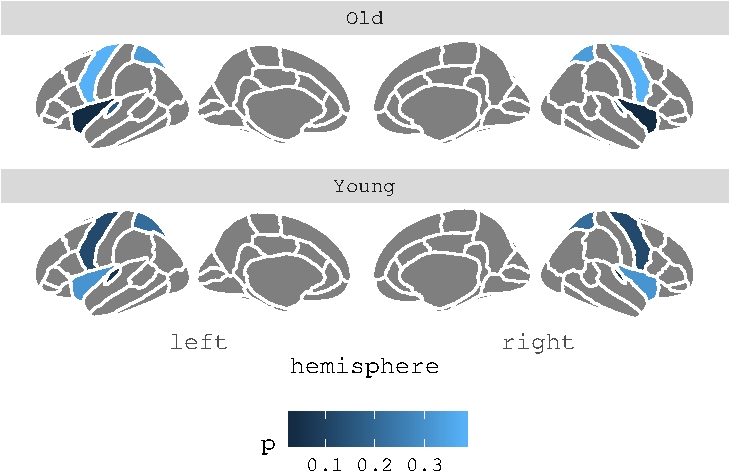
\includegraphics{draft_1_files/figure-latex/datasupp3-1.pdf}

Depending on what type of column is used for fill (continuous or discrete),
you can also use the differenct \texttt{scales} to alter the colours.

\begin{Shaded}
\begin{Highlighting}[]
\KeywordTok{ggseg}\NormalTok{(}\DataTypeTok{.data =}\NormalTok{ someData, }\DataTypeTok{atlas=}\NormalTok{dkt, }
      \DataTypeTok{colour=}\StringTok{"white"}\NormalTok{, }\DataTypeTok{position=}\StringTok{"stacked"}\NormalTok{,}
      \DataTypeTok{mapping=}\KeywordTok{aes}\NormalTok{(}\DataTypeTok{fill=}\NormalTok{p)) }\OperatorTok{+}
\StringTok{  }\KeywordTok{facet_wrap}\NormalTok{(}\OperatorTok{~}\NormalTok{AgeG, }\DataTypeTok{ncol=}\DecValTok{2}\NormalTok{) }\OperatorTok{+}
\StringTok{  }\KeywordTok{theme_dark}\NormalTok{() }\OperatorTok{+}
\StringTok{  }\KeywordTok{theme}\NormalTok{(}\DataTypeTok{legend.position =} \StringTok{"bottom"}\NormalTok{,}
        \DataTypeTok{axis.text =} \KeywordTok{element_blank}\NormalTok{(),}
        \DataTypeTok{axis.title =} \KeywordTok{element_blank}\NormalTok{()}
\NormalTok{        ) }\OperatorTok{+}
\StringTok{  }\KeywordTok{scale_fill_gradient2}\NormalTok{(}\DataTypeTok{high=}\StringTok{"goldenrod"}\NormalTok{,}
                       \DataTypeTok{low=}\StringTok{"firebrick"}\NormalTok{,}
                       \DataTypeTok{na.value=}\StringTok{"transparent"}\NormalTok{)}
\end{Highlighting}
\end{Shaded}

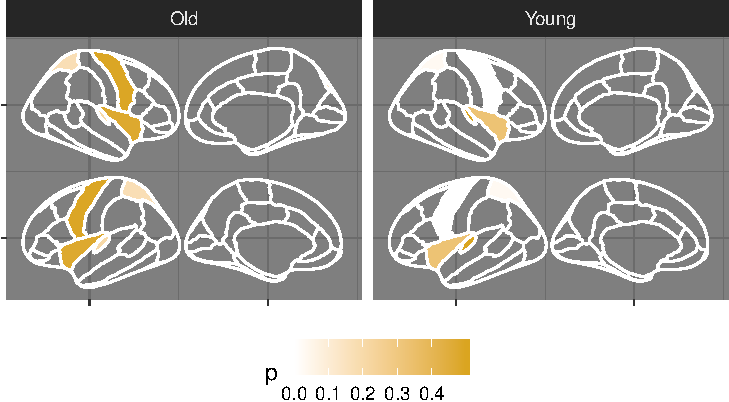
\includegraphics{draft_1_files/figure-latex/datasupp5-1.pdf}

All the consepts described above also work with the \texttt{aseg} atlas for subcrotical structures, except arguments to see only one hemisphere or lateral or medial surfaces, as these arguments do not make sense for this atlas.
Again, inspecting the atlas data directly will be of aid when preparing data to use with the atlas
\small

\begin{Shaded}
\begin{Highlighting}[]
\NormalTok{aseg}
\end{Highlighting}
\end{Shaded}

\begin{verbatim}
## # A tibble: 34 x 6
##    atlas area            hemi  side  label                ggseg            
##    <chr> <chr>           <chr> <chr> <fct>                <list>           
##  1 aseg  <NA>            right axial <NA>                 <tibble [808 x 5~
##  2 aseg  <NA>            left  axial <NA>                 <tibble [1,014 x~
##  3 aseg  thalamus proper left  axial Left-Thalamus-Proper <tibble [56 x 5]>
##  4 aseg  thalamus proper left  axial Right-Thalamus-Prop~ <tibble [56 x 5]>
##  5 aseg  thalamus proper right axial Left-Thalamus-Proper <tibble [61 x 5]>
##  6 aseg  thalamus proper right axial Right-Thalamus-Prop~ <tibble [61 x 5]>
##  7 aseg  lateral ventri~ right axial Left-Lateral-Ventri~ <tibble [66 x 5]>
##  8 aseg  lateral ventri~ right axial Right-Lateral-Ventr~ <tibble [66 x 5]>
##  9 aseg  hippocampus     left  axial Left-Hippocampus     <tibble [47 x 5]>
## 10 aseg  hippocampus     left  axial Right-Hippocampus    <tibble [47 x 5]>
## # ... with 24 more rows
\end{verbatim}

\normalsize

\begin{Shaded}
\begin{Highlighting}[]
\KeywordTok{ggseg}\NormalTok{(}\DataTypeTok{atlas=}\StringTok{"aseg"}\NormalTok{, }\DataTypeTok{mapping=}\KeywordTok{aes}\NormalTok{(}\DataTypeTok{fill=}\NormalTok{area))}
\end{Highlighting}
\end{Shaded}

\begin{figure}
\centering
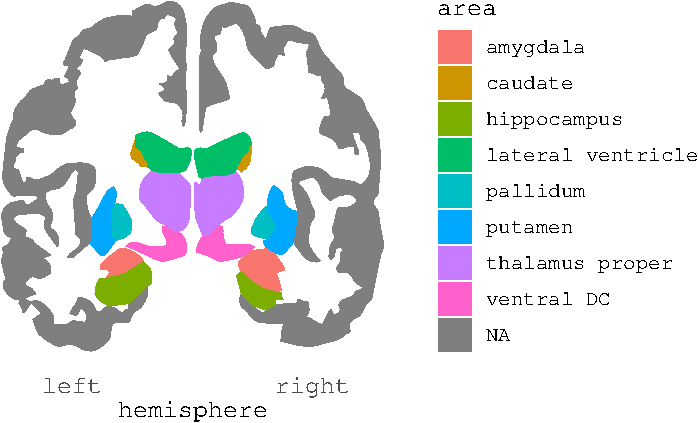
\includegraphics{draft_1_files/figure-latex/atlases-1.pdf}
\caption{\label{fig:atlases}The first 10 rows of the \texttt{aseg} dataset, that has some specific differences from the dkt, like missing the option to not view both hemispheres, as the plot would be hard to understand that way.}
\end{figure}

\hypertarget{plotting-3d-mesh-data}{%
\subsection{Plotting 3D mesh data}\label{plotting-3d-mesh-data}}

Creating plots of the brain as 2-dimensional can at times make it difficult to properly understand where an atlas segment is located in the true 3-dimensional brain.
This is particularly true when looking within the brain as subcortical structures or white matter tracts.
To provide the option of viewing and printing the plots in 3-dimensional space, another function was created using plotly \citep{plotly}.
The data is somewhat more complex than the 2D ggplot polygon version \texttt{ggseg}, as it includes options for brain inflation, glass brains and much more, to ease viewing and understanding.
Another positive effect of basing this function on plotly, is the interactivity of the plot, which also makes it nice for public dissemination.
A lot of credit goes to A.M.Winkler and his Brainder (\citet{brainder}) work, which supplied us with the first examples of going from Freesurfer \texttt{.srf}-files to \texttt{.ply}-files, and whose scripts massively aided us in making this work.

The function \texttt{ggseg3d()}, is based in the plotly, it is recommended to get a little familiarized with with plotly (\citet{plotly}).

Out-of-the-box, \texttt{ggseg3d()} works without supplying any extra information, and plots the \texttt{dkt\_3d} atlas in `LCBC' surface.
The `LCBC' surface is the white matter surface, inflated in 10 steps, to increase visibility within folds of the brain, while still maintining curvature to indicate where folds have been.
All \texttt{{[}...{]}\_3d} atlases have a built in \texttt{colour} column for default colour plotting of the segments.

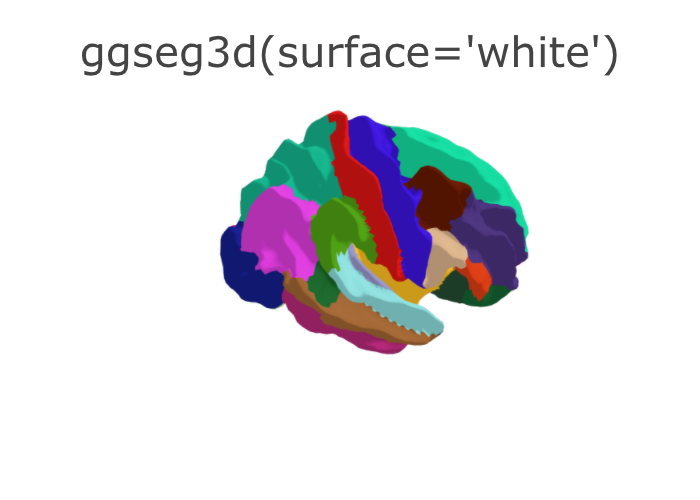
\includegraphics[width=0.3\linewidth]{png/ggseg3d_white}
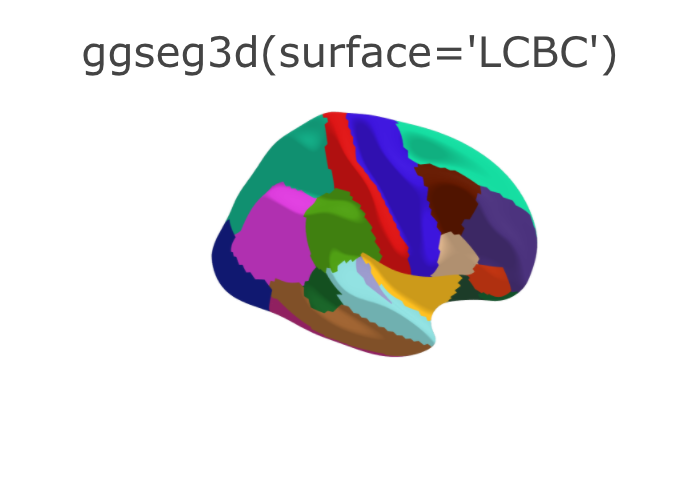
\includegraphics[width=0.3\linewidth]{png/ggseg3d}
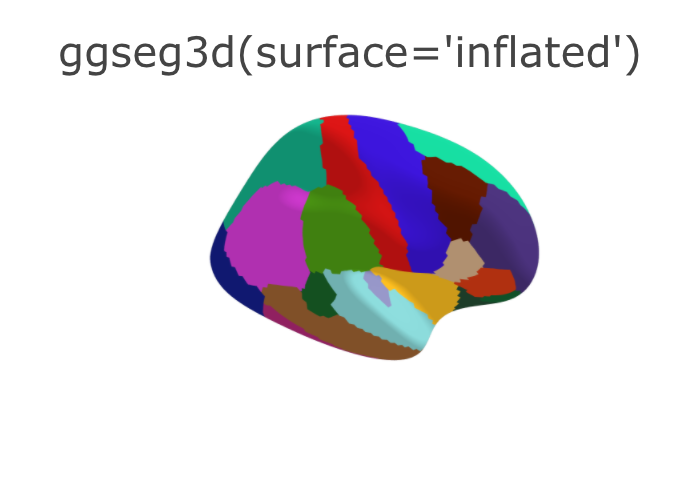
\includegraphics[width=0.3\linewidth]{png/ggseg3d_inflated}

The cortical atlas data is stored in nested tibbles, which have datasets for three different surfaces and the two hemispheres.
The `data'-column within includes all necessary information to \texttt{ggseg3d()} to create a mesh-plot.
\small

\begin{Shaded}
\begin{Highlighting}[]
\NormalTok{dkt_3d}
\end{Highlighting}
\end{Shaded}

\begin{verbatim}
## # A tibble: 6 x 4
##   atlas  surf     hemi  ggseg_3d         
##   <chr>  <chr>    <chr> <list>           
## 1 dkt_3d inflated left  <tibble [36 x 8]>
## 2 dkt_3d inflated right <tibble [36 x 8]>
## 3 dkt_3d LCBC     left  <tibble [36 x 8]>
## 4 dkt_3d LCBC     right <tibble [36 x 8]>
## 5 dkt_3d white    left  <tibble [36 x 8]>
## 6 dkt_3d white    right <tibble [36 x 8]>
\end{verbatim}

\normalsize

To grab all the data for a surface and hemisphere, you should reduce the data to one line, and then \texttt{unnest()}

\begin{Shaded}
\begin{Highlighting}[]
\NormalTok{dkt_3d }\OperatorTok\StringTok{ }
\StringTok{  }\KeywordTok{filter}\NormalTok{(surf }\OperatorTok{==}\StringTok{ "inflated"} \OperatorTok{&}\StringTok{ }\NormalTok{hemi }\OperatorTok{==}\StringTok{ "right"}\NormalTok{) }\OperatorTok\StringTok{ }
\StringTok{  }\KeywordTok{unnest}\NormalTok{(ggseg_3d) }\OperatorTok\StringTok{ }
\StringTok{  }\KeywordTok{select}\NormalTok{(}\OperatorTok{-}\NormalTok{lobe, }\OperatorTok{-}\NormalTok{acronym)}
\end{Highlighting}
\end{Shaded}

\begin{verbatim}
## # A tibble: 36 x 9
## atlas surf hemi area colour mesh label roi annot
## <chr> <chr> <chr> <chr> <chr> <list> <chr> <chr> <chr>
## 1 dkt_3d infla~ right <NA> <NA> <list~ rh_medial~ 0001 medialwa~
## 2 dkt_3d infla~ right banks supe~ #1964~ <list~ rh_bankss~ 0002
bankssts
## 3 dkt_3d infla~ right caudal ant~ #7D64~ <list~ rh_caudal~ 0003
caudalan~
## 4 dkt_3d infla~ right caudal mid~ #6419~ <list~ rh_caudal~ 0004
caudalmi~
## 5 dkt_3d infla~ right corpus cal~ <NA> <list~ rh_corpus~ 0005
corpusca~
## 6 dkt_3d infla~ right cuneus #DC14~ <list~ rh_cuneus 0006 cuneus
## 7 dkt_3d infla~ right entorhinal #DC14~ <list~ rh_entorh~ 0007
entorhin~
## 8 dkt_3d infla~ right fusiform #B4DC~ <list~ rh_fusifo~ 0008
fusiform
## 9 dkt_3d infla~ right inferior p~ #DC3C~ <list~ rh_inferi~ 0009
inferior~
## 10 dkt_3d infla~ right inferior t~ #B428~ <list~ rh_inferi~ 0010
inferior~
## # ... with 26 more rows
\end{verbatim}

\hypertarget{external-data-supply}{%
\subsubsection{External data supply}\label{external-data-supply}}

Particularly notice the \texttt{mesh} column, which is a list column of lists.
In there is all the 6 vectors needed to create the mesh of the tri-surface plot.
You'll also need to notice the \texttt{label}, \texttt{annot} and \texttt{area} columns, which are likely the columns you will be matching on when proviging with your own data for colours.
You need to be meticulous when fixing your data, be sure it matches.
The function \emph{should} give you a warning if it's struggling to match something.

The column you want to use for colour, needs to be supplied to the \texttt{colour} option, and you'll likely want to supply it to the \texttt{text} option, as this will add another line to the plotly hover information.

\begin{Shaded}
\begin{Highlighting}[]
\NormalTok{someData =}\StringTok{ }\NormalTok{dkt_3d }\OperatorTok\StringTok{ }
\StringTok{  }\KeywordTok{filter}\NormalTok{(surf }\OperatorTok{==}\StringTok{ "inflated"} \OperatorTok{&}\StringTok{ }
\StringTok{         }\NormalTok{hemi }\OperatorTok{==}\StringTok{ "right"}\NormalTok{) }\OperatorTok\StringTok{ }
\StringTok{  }\KeywordTok{unnest}\NormalTok{(ggseg_3d) }\OperatorTok\StringTok{ }
\StringTok{  }\KeywordTok{select}\NormalTok{(area) }\OperatorTok\StringTok{ }
\StringTok{  }\KeywordTok{na.omit}\NormalTok{() }\OperatorTok\StringTok{ }
\StringTok{  }\KeywordTok{mutate}\NormalTok{(}\DataTypeTok{p =} \KeywordTok{sample}\NormalTok{(}\KeywordTok{seq}\NormalTok{(}\DecValTok{0}\NormalTok{,.}\DecValTok{5}\NormalTok{, }\DataTypeTok{length.out =} \DecValTok{100}\NormalTok{ ), }\KeywordTok{nrow}\NormalTok{(.)) }\OperatorTok\StringTok{ }
\StringTok{           }\KeywordTok{round}\NormalTok{(}\DecValTok{2}\NormalTok{)) }
  
  \KeywordTok{ggseg3d}\NormalTok{(}\DataTypeTok{.data =}\NormalTok{ someData, }\DataTypeTok{atlas =}\NormalTok{ dkt_3d, }\DataTypeTok{colour =} \StringTok{"p"}\NormalTok{, }\DataTypeTok{text =} \StringTok{"p"}\NormalTok{)}
\end{Highlighting}
\end{Shaded}

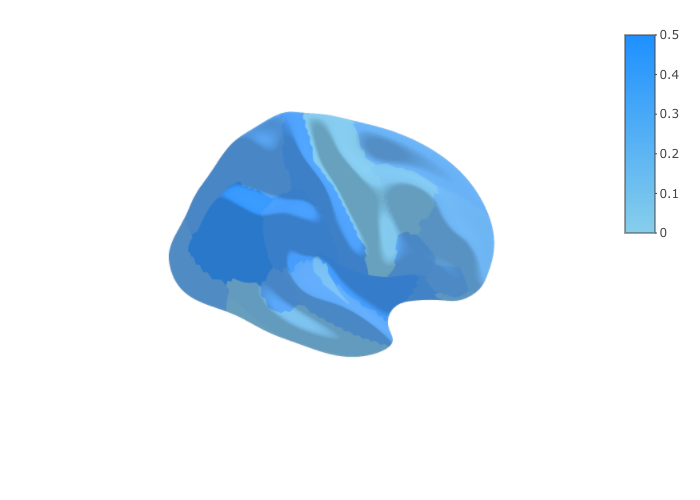
\includegraphics[width=0.4\linewidth]{png/ggseg3d_data}

\hypertarget{colours}{%
\subsubsection{Colours}\label{colours}}

You can provide custom colour palettes either in hex or R-names.
Colours will be evenly spaced when creating the colour-scale, and you may provide as many colours as you wish.

\begin{Shaded}
\begin{Highlighting}[]
  \KeywordTok{ggseg3d}\NormalTok{(}\DataTypeTok{.data =}\NormalTok{ someData, }\DataTypeTok{atlas =}\NormalTok{ dkt_3d, }
          \DataTypeTok{colour =} \StringTok{"p"}\NormalTok{, }\DataTypeTok{text =} \StringTok{"p"}\NormalTok{, }
          \DataTypeTok{palette =} \KeywordTok{c}\NormalTok{(}\StringTok{"#ff0000"}\NormalTok{, }\StringTok{"#00ff00"}\NormalTok{, }\StringTok{"#0000ff"}\NormalTok{))}
\end{Highlighting}
\end{Shaded}

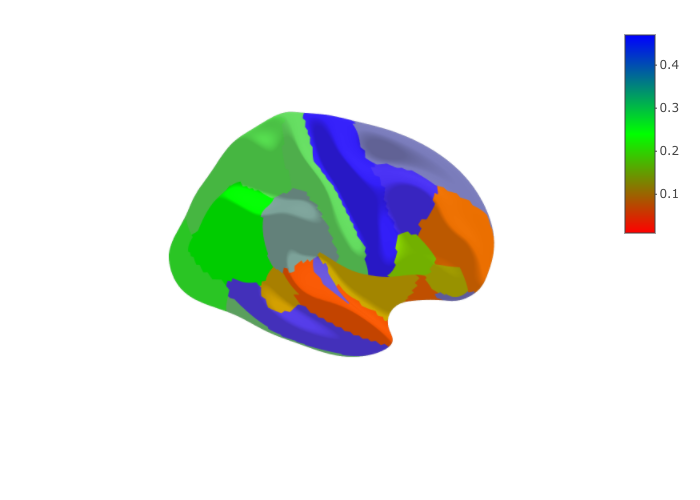
\includegraphics[width=0.4\linewidth]{png/ggseg3d_colour}

If you want to alter the colour of \texttt{NA} regions, supply \texttt{na.colour}, either as HEX colour or colour name.
This option only takes a single colour.

\begin{Shaded}
\begin{Highlighting}[]
  \KeywordTok{ggseg3d}\NormalTok{(}\DataTypeTok{.data =}\NormalTok{ someData, }\DataTypeTok{atlas =}\NormalTok{ dkt_3d, }
          \DataTypeTok{colour =} \StringTok{"p"}\NormalTok{, }\DataTypeTok{text =} \StringTok{"p"}\NormalTok{, }
          \DataTypeTok{na.colour =} \StringTok{"black"}\NormalTok{, }\DataTypeTok{camera=}\StringTok{"medial"}\NormalTok{)}
\end{Highlighting}
\end{Shaded}

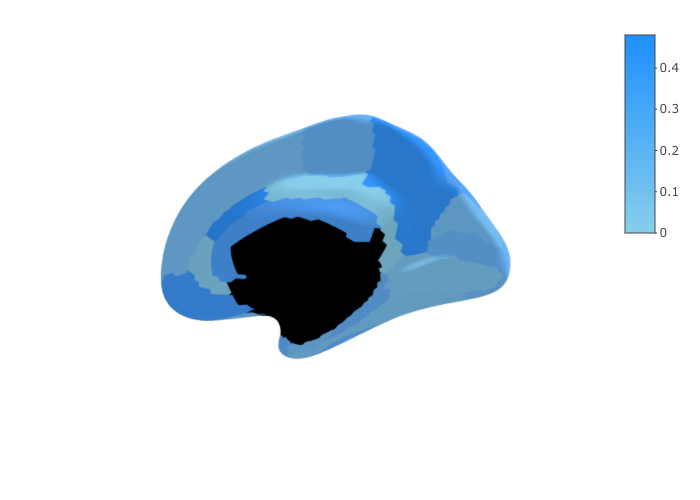
\includegraphics[width=0.4\linewidth]{png/ggseg3d_nacolour}

If you are plotting the sub-cortical structures, you might want to reduce the opacity of the \texttt{NA} structures, so that you can see the more medial structures.
You may also want to add the \texttt{glassbrain} option, any value above 0 and up to 1 increases the opacity of a glass brain overlay.
The glassbrain option provides a frame of reference for the subcortical structures, and as such it is recommended to add this when viewing these structures.
There are three glassbrain options, controlling the opacity, which hemispheres to add, and the colour.

\begin{Shaded}
\begin{Highlighting}[]
\NormalTok{somData_aseg =}\StringTok{ }\NormalTok{aseg_3d }\OperatorTok\StringTok{ }
\StringTok{  }\KeywordTok{unnest}\NormalTok{() }\OperatorTok\StringTok{ }
\StringTok{  }\KeywordTok{select}\NormalTok{(label) }\OperatorTok\StringTok{ }
\StringTok{  }\KeywordTok{filter}\NormalTok{(}\OperatorTok{!}\KeywordTok{grepl}\NormalTok{(}\StringTok{"Ventricle|Putamen"}\NormalTok{, label)) }\OperatorTok\StringTok{ }
\StringTok{  }\KeywordTok{mutate}\NormalTok{(}\DataTypeTok{p =} \KeywordTok{seq}\NormalTok{(}\DecValTok{1}\NormalTok{, }\KeywordTok{nrow}\NormalTok{(.))) }

  \KeywordTok{ggseg3d}\NormalTok{(}\DataTypeTok{.data =}\NormalTok{ somData_aseg, }\DataTypeTok{atlas =}\NormalTok{ aseg_3d, }
          \DataTypeTok{colour =} \StringTok{"p"}\NormalTok{, }\DataTypeTok{text =} \StringTok{"p"}\NormalTok{, }
          \DataTypeTok{na.alpha=} \FloatTok{.5}\NormalTok{, }\DataTypeTok{glassbrain =} \FloatTok{.5}\NormalTok{, }
          \DataTypeTok{glassbrain_hemisphere =} \StringTok{"left"}\NormalTok{)}
\end{Highlighting}
\end{Shaded}

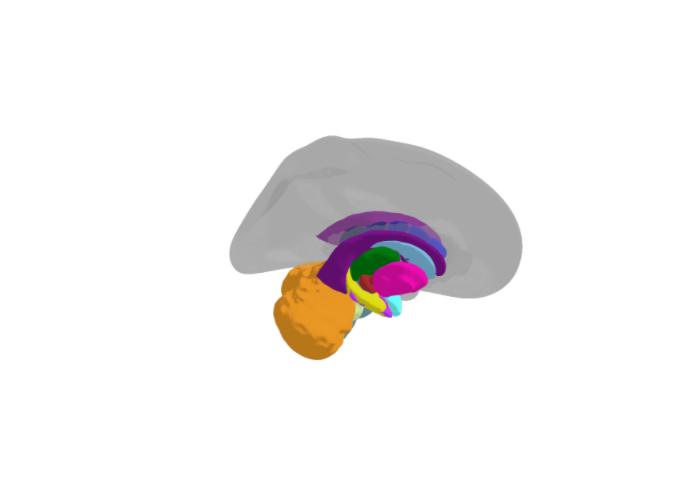
\includegraphics[width=0.4\linewidth]{png/ggseg3d_glass}

There are many plotly options that may help you adapt the plot to look the way you wish.
In addition to Carson Sievert's book on plotly in R (\citeyearpar{plotly}) we recommend resources for modifying axes in 3D plots (\citet{plotly-ax}), the basic introduction to tri-surface plots (\citet{plotly-tri}), and this tutorial on tri-surface plots with plotly in R (\citet{plotly-trisurf}).

\hypertarget{summary}{%
\section{Summary}\label{summary}}

The aim of the \texttt{ggseg}-package is to aid researchers easily disseminate analysis results in an easier and more stream-lined fashion.
This tutorial should provide instructions on how to use the main package functions, and cover the most commonly used options.
The two main functions in the package, \texttt{ggseg()} and \texttt{ggseg3d()}, create polygon and mesh-plots of brain atlases, using the accompanying package data.
In addition to the two default atlases available in \texttt{ggseg}, the \texttt{ggsegExtra} package includes 12 more atlases.
We encourage users of this package to contribute more atlases they find uses for, and help build an extensive repository of brain atlases.

\hypertarget{author-contributions}{%
\section{Author Contributions}\label{author-contributions}}

Didac Vidal-Piñeiro generated the idea for the plotting tool, and the initial scripts that made the plots.
He has also been responsible for converting images from neuroimaging software into the type of data necessary for plotting polygons and mesh plots in R.
Athanasia M. Mowinckel adapted the initial scripts and made the functions into package format and making the functions more user-friendly.
She also was responsible for adding the mesh-plot functionality through plotly, and developing the pipeline for making that possible.
A. M. Mowinckel wrote the first draft of the paper, and both have since critically edited it.

\hypertarget{conflicts-of-interest}{%
\section{Conflicts of Interest}\label{conflicts-of-interest}}

The authors declare that there were no conflicts of interest with respect to the authorship or the publication of this article.

\hypertarget{acknowledgements}{%
\section{Acknowledgements}\label{acknowledgements}}

We also thanks John Muschelli for his initial improvements in the package code and preparing it for incorporation in neuroconductor (\citeyearpar{neuroconductor}), and Richard Beare for submitting the first community created atlas, and providing helpful comments to the base code.

\hypertarget{funding}{%
\section{Funding}\label{funding}}

This work is funded by EU Horizon 2020 Grant `Healthy minds 0-100 years: Optimising the use of European brain imaging cohorts (Lifebrain)', with grant agreement number 732592.

\hypertarget{prior-versions}{%
\section{Prior versions}\label{prior-versions}}

Some of the content presented here also apprears in the package vignette of \texttt{ggseg}, which may be accessed through R or in the package website (\citet{ggseg}).
Athanasia Monika Mowinckel also has several tutorials on her blog regarding ggseg creationg and functionality (\citet{ggsegAnim}, \citet{ggsegIntro}).

\renewcommand\refname{References}
\bibliography{references.bib}



\end{document}
